
\section{General Results and Descriptive Statistics}
\label{sec:descr-stat}

% \sm{move here ``Crowd judging''?}

\subsection{Crowd Judging}
\label{sec:crowd-judging}

%\myparagraph{Crowd Judging:}
As detailed in Table~\ref{tab:descr-stat}, with 7,059 units comprised
of 8 documents each, we collected more than 50,000 judgments in total,
at a cost of around $\$1,700$ (CrowdFlower fees included).
This is in the order of magnitude of $\$0.4$ for each document, which
is broadly competitive when compared with the cost of TREC assessors
or other similar crowdsourcing initiatives; for example, according to
\citet[Footnote~2]{Alonso:2012}, gathering ordinal scale judgments
cost around $\$0.1$ per document.
However, the comparison is more favorable when considering that in our
experiments 10 redundant judgments per document are collected, and the
\nkn and \hkh documents receive multiple judgments, whereas in Alonso
and Mizzaro's work only 5 redundant judgments were collected, and
there was nothing similar to our \nkn vs. 
\hkh check.
We return to the cost issues in more detail in 
Section~\ref{sec:how-many-workers}, where the number of repeat
judgments that are required for stable ME estimates is investigated.  

In total, 1481 workers participated in our experiments. 
Since it was impossible for a worker to perform the task twice (or
more) for each topic, each worker could complete between 1
(around 30\% of the workers did so) and 18 (less than 1\% of the
workers) tasks.
As is usual in similar crowdsourcing experiments, the distribution
of the number of tasks for a worker resembles a power law, although
with only 18 tasks at maximum it is difficult to be precise on that.
Finally, workers tend to work in sessions: when they complete a topic they
either leave after that, or sometimes they complete a subsequent topic
straight away---they much more rarely leave and come back later to
do another.
% In Section~\ref{sec:comment-analysis} we consider the effect that this
% has on 
% the comments left by the workers.
% \fs{Check that this is actually included in the final version of
% Section~\ref{sec:comment-analysis}.}

\subsection{Score Distribution}
\label{sec:score-distribution}

\begin{figure}[t]
  \centering
  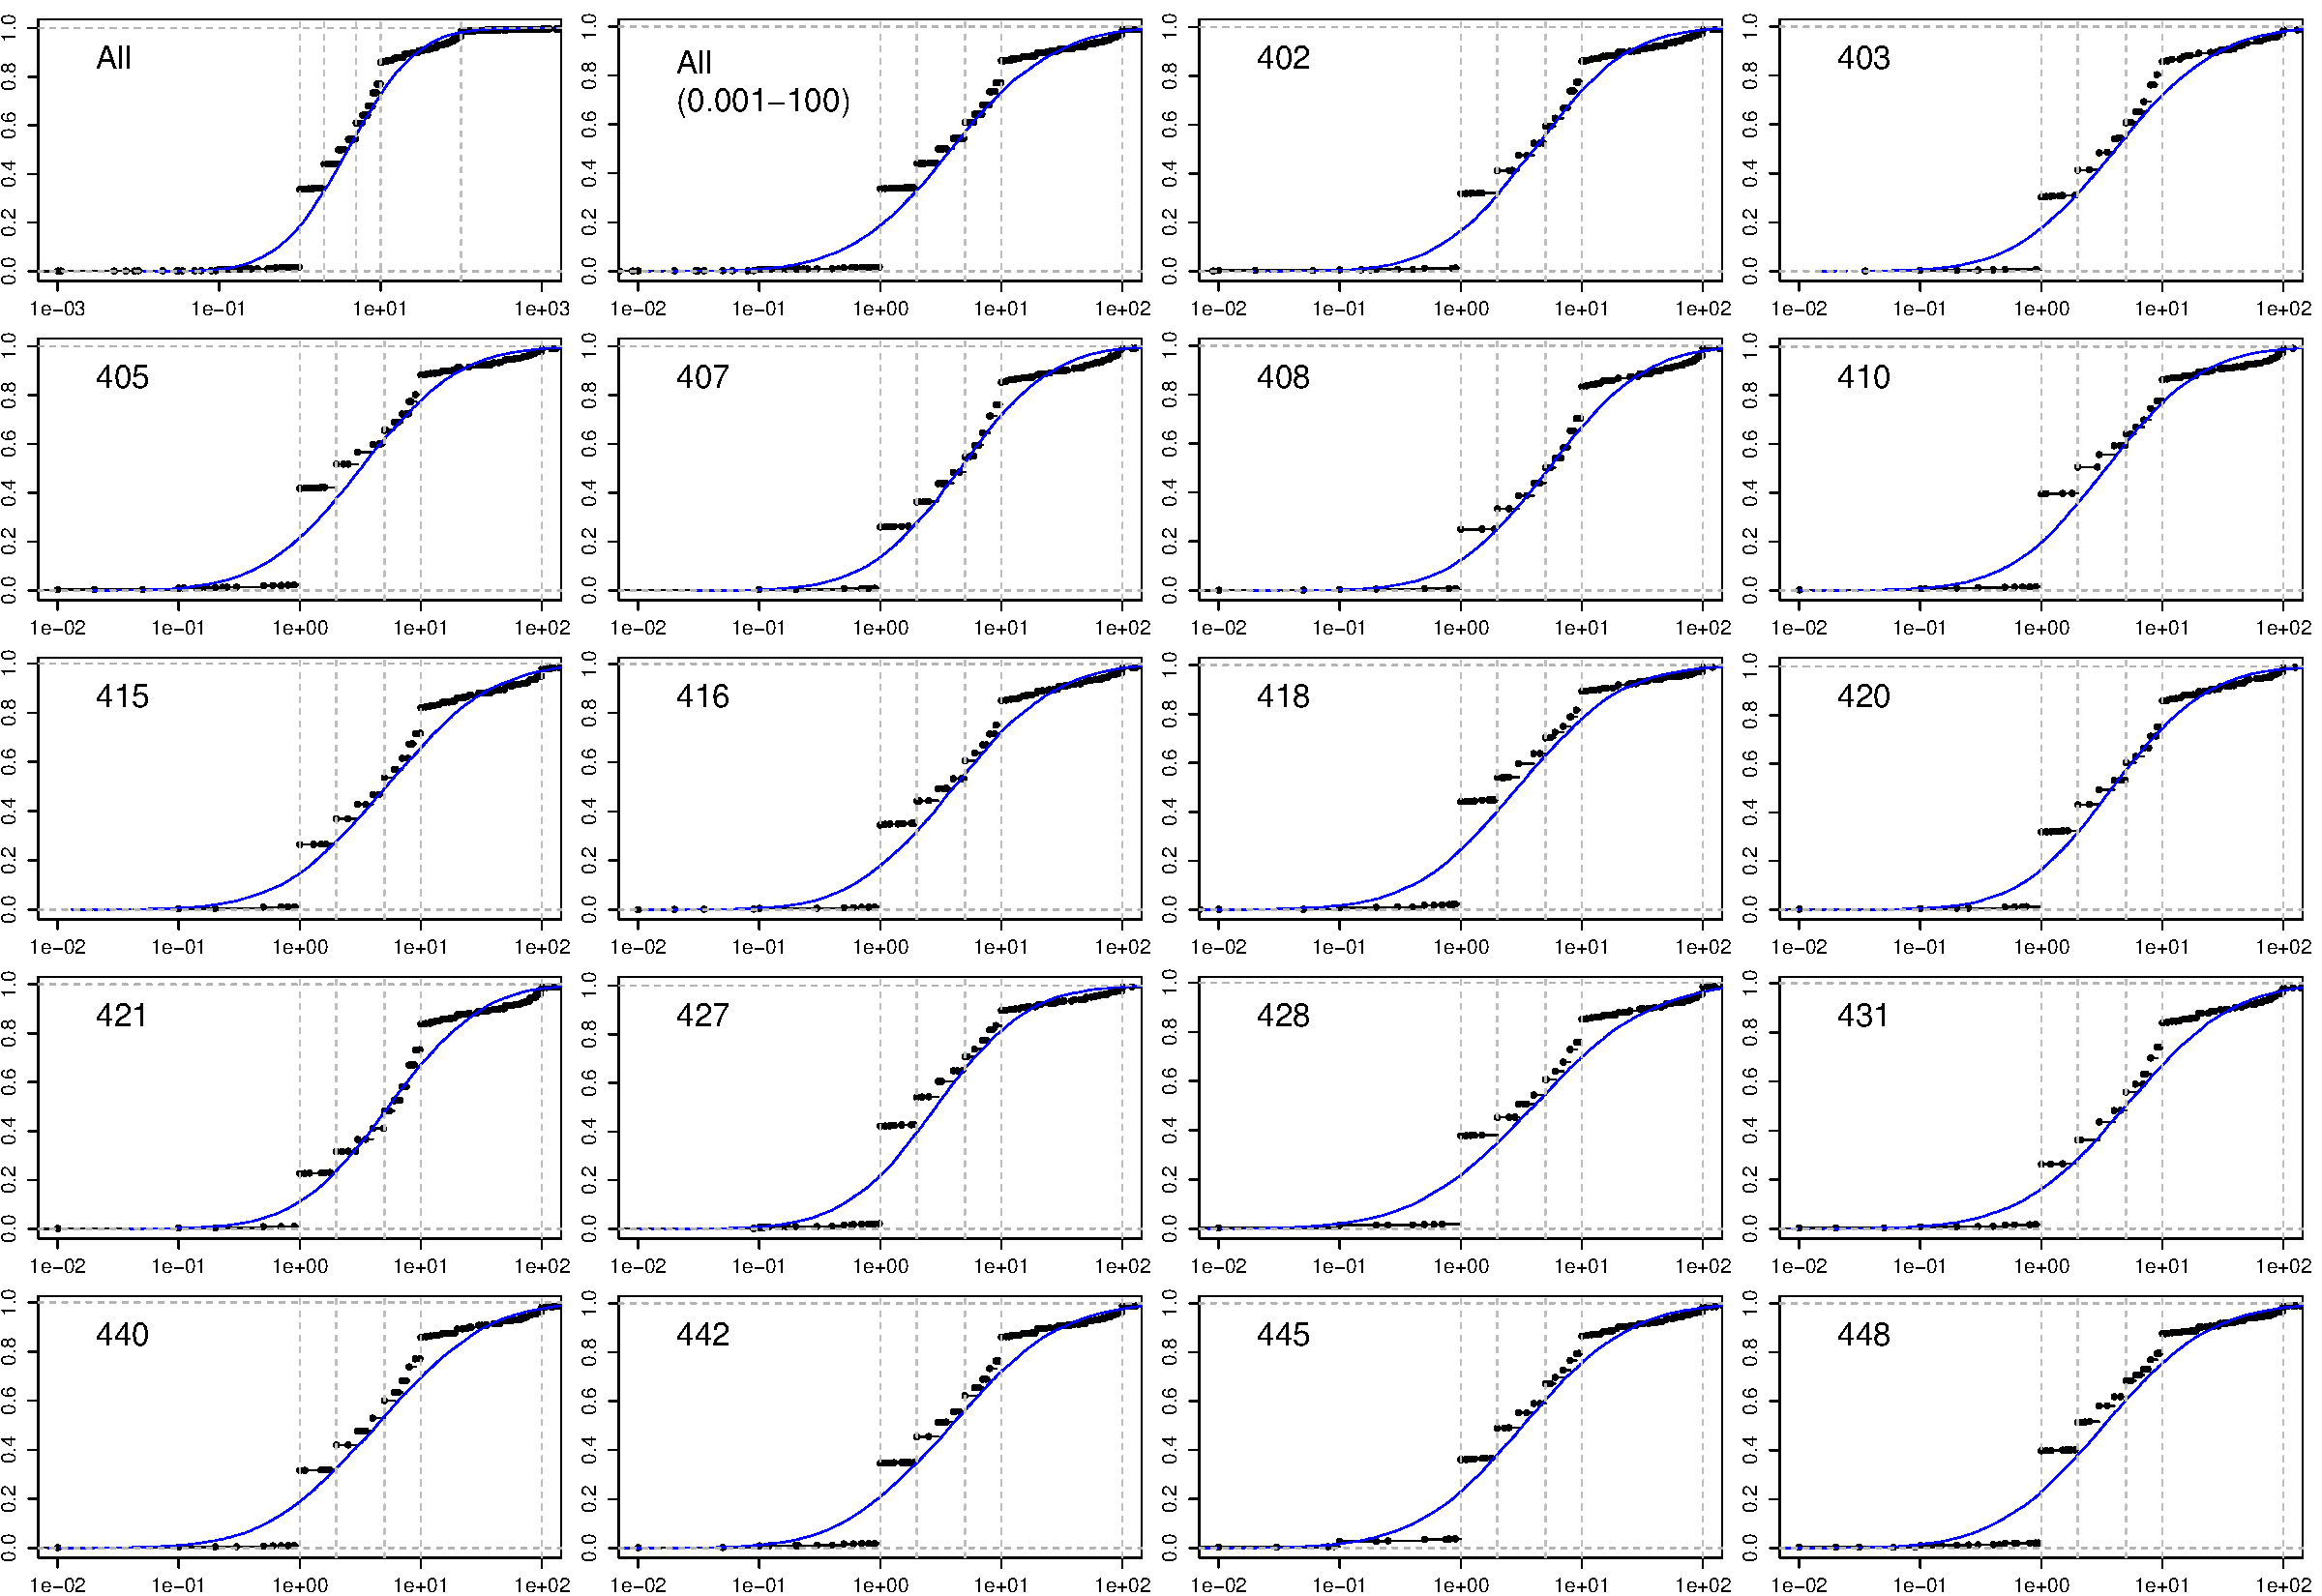
\includegraphics[width=\linewidth,page=1]{figs/MEscores.pdf}
  \caption{Cumulative distribution functions of raw ME scores for each topic 
(labelled in the top left of each panel) for all scores in the range
0.01 to 100. Black dots are gathered scores and the blue line in each panel is a 
fitted log-normal curve. The x axis is a log scale. 
Vertical dashed lines are at 1, 2, 5 and 10.}
  \label{fig:ME-raw-scores}
\end{figure}

Magnitude estimation scores should be approximately
log-normal~\citep{Mar74,moskowitz:1977}. 
%\sm{ks test on the logs does not indicate normality but...}
Figure~\ref{fig:ME-raw-scores} shows the situation for our data, 
plotting the Cumulative Distribution Functions (CDFs) of:
all the scores (top left), all the scores in the $0.001$-$100$ range
(which includes about 99.5\% of the scores), and the scores for each
topic. 
The continuous blue lines are fitted log-normal distributions with the
same mean and standard deviation of the corresponding data.  
From the figure it is clear that the log-normal distribution is a
reasonable approximation of the raw data. 
Differences are generally due to a \emph{round number tendency}
\cite{moskowitz:1977}: in general, people expressing magnitudes using
a numeric scale tend to use some specific values more than others, for
instance integer numbers and powers of ten. 
From the figure it can be seen that our workers tended to use
especially 1, 2, 5, and 10 (the values where ``steps'' can be seen on
the CDF curves --- see the gray vertical dashed lines on the charts),
and also quite a lot of 3, 4, 5, 6 7, 8, 9, 20, 30, 40, 50, 60, 70,
80, 90, and 100. 
The breakdowns on single topics show that topics do have an effect
(for instance, in topics 418 and 421 the scores up to~1 included
account for about 44\% and 23\% of the values respectively), although
the general trend is very similar, as is again demonstrated by the
fitted log-normal distributions.
Topic means ranged from 7.9 to 12.9, and topic standard deviations ranged
from 17.5 to 23.2.

% raw scores means
%      402       403      405       407       408       410       415 416 
%10.013831 10.014614 8.595449 11.392839 12.990020 10.409096 12.467627 10.079280 
%      418       420       421       427       428       431       440 442 
%8.069978 10.199124 12.662327  7.903648 11.308172 11.505793 10.237795 10.398175 
%      445       448 
%9.081898  9.197152 

% standard deviations of raw scores
%     402      403      405      407      408      410      415      416 
%19.20965 19.59646 17.96137 21.16121 23.24930 21.54687 22.91172 19.67080 
%     418      420      421      427      428      431      440      442 
%17.87859 19.53965 22.58363 17.53647 22.80461 21.33762 20.23102 21.00615 
%     445      448 
%18.92293 19.69537 

\subsection{Score Normalization and Aggregation} 
\label{sec:score-normalization}

Magnitude estimation is a highly flexible process, with observers being
free to assign any positive number, including fractions, as a rating of
the intensity of a presented stimulus.
The key requirement is that the ratio of the numbers should reflect the
ratio of the differences in perception between stimulus intensities.
As the stimuli are presented in a randomized order, and observers are
free to assign a number of their choice to the first presented item, it
is natural that different participants may make use of different parts
of the positive number space.
Magnitude estimation scores are therefore normalized, to adjust for
these differences.
Geometric averaging is the recommended approach for the normalization
of magnitude estimation scores~\cite{Ges97,McG03,moskowitz:1977}, and
was applied in our data analysis.
Recall that for a given search topic, participants made magnitude
estimation judgments for groups of eight documents (a unit).
To normalize the scores, first the log of each raw score, $s_i$, is
taken. Next, the arithmetic mean of these log scores is calculated for
each {\emph{unit}} of 8 documents, and for the {\emph{topic}} as a
whole. 
Each individual log score is then adjusted by the unit and topic means,
and the exponent is taken of the resulting quantity, giving the final
normalized score 
\begin{align}
  s'_i &= e^{\log(s_i) - \mu(\log(\mathnormal{unit})) + \mu
           (\log(\mathnormal{topic})) } \label{eq:1}
\end{align}
% To normalize the scores, first the log of each raw score, $s_i$, is
% taken.
% Next, the arithmetic mean of these log scores is calculated for each
% unit of 8 documents ($\mu_u$), and for the topic as a whole ($\mu$).
% Each individual log score is then adjusted by the unit and topic means,
% and the exponent is taken of the resulting quantity, giving the final
% normalized score 
% \begin{align}
% s'_i &= \exp(\log(s_i) - \mu_u + \mu ). \label{eq:1} 
% \end{align}
An alternative equivalent formalization is: 
\begin{align}
s'_i &= s_i \cdot \frac{\gamma}{\gamma_u}, 
\label{eq:2}
\end{align}
where $\gamma_u$ is the geometric mean for each unit and $\gamma$ is
the geometric mean for the topic as a whole.
The log transformation is theoretically motivated by the fact that
magnitude estimation scores of perceived stimulus intensities have been
found to be approximately log-normal, which was the case in our data as
shown in Section~\ref{sec:score-distribution}. Intuitively,
normalization by geometric averaging means that the raw magnitude
estimation scores are moved along the number line, both in terms of
location and spread, and the individual differences in scale are
nullified.
For example, as shown by both 
\citet{moskowitz:1977} and  
\citet{McG03}, 
if two judges assigned scores of \{1, 2, 3, 4\} and \{10, 20, 30, 40\}
to the same set of four items, respectively, then the normalized values
would be identical in the two cases, as can be easily verified by
applying either Equation~(\ref{eq:1}) or~(\ref{eq:2}).
Importantly, normalization through geometric averaging has the property
of preserving the ratios of the original scores, the essential feature
of the magnitude estimation process.
%\sm{So, in the example above, 2, 3, 4, 5 would be normalized into something different,  as the ratios are different.}
%
\begin{figure}[tp]
  \centering
  \includegraphics[width=\linewidth,page=2]{figs/MEscores.pdf}
  \caption{CDFs of normalized ME scores using the
    same style as Figure~\ref{fig:ME-raw-scores}.
  \label{fig:ME-norm-scores}}
\end{figure}

Other normalizations have been proposed, 
for example using the median or the arithmetic mean instead of the
geometric mean (especially when zero is an allowed score, so the
geometric mean cannot be used)~\citet{moskowitz:1977}.
Other approaches include carrying out an additional calibration task
that is aimed at understanding the differences in individual scales;
in our scenario, this might be implemented by exploiting the \nkn and
\hkh documents, or in a more implicit way by relying on the maximal
and minimal scores expressed by each worker.

Unless otherwise noted, all analysis reported in this paper uses
magnitude estimation scores normalized by geometric averaging.
Geometric averaging normalization is in principle adequate since, as
we have discussed, our scores are approximately log-normal and they do
not include zero. 
Figure~\ref{fig:ME-norm-scores} shows the distribution of scores after
normalization which are similar to 
Figure~\ref{fig:ME-raw-scores}.
It can be noted how the normalization has the effect of smoothing the
scores (the round number tendency disappears, since each score is moved by a
quantity which is different for each worker) and of making them even
more log-normal.
%\aht{Does the ks test show (log) normal for this one?}

%%%?\begin{figure}[tp]
%%%?  \centering
%%%?  \includegraphics[width=\linewidth]{figs/MEscores-boxplot.png}
%%%?  \caption{Normalized  ME scores (y log scale) per topic.
%%%?  \label{fig:ME-norm-scores-boxplot}}
%%%?\end{figure}
%%%?
%%%?The boxplots of the normalized ME scores are shown in
%%%?Figure~\ref{fig:ME-norm-scores-boxplot}: the topic differences are
%%%?more clear here, and \sm{statsig test? 
%%%?  topic difficulty blahblahblah??} 
%%%?\fs{I suggest that we leave this fig out. 
%%%?  The per-topic distributions are avaliable (although split by Sorm
%%%?  level) in the other fig (two figs on) anyway, and IMO it would be
%%%?  better to *not* mention ``topic difficulty'', except perhaps as
%%%?  future work, and then do it properly as future work.} 
%%%?\sm{I leave it by now but I rather agree. 
%%%?  Andrew?}

% \subsection{Score aggregation[.5pg]}
% \label{sec:score-aggregation}

The problem of aggregating several ME scores for the same item also
needs some attention. 
For each topic-document pair we collected at least 10 ME scores, by 10
different workers (many more for the \nkn and \hkh documents). 
In the following we will primarily use the \emph{median} of the normalized ME
scores for a topic-document pair, although again alternatives are available at this step,
such as using the arithmetic mean or
the geometric mean of obtained ME scores~\cite{moskowitz:1977}. 
We briefly examine the effect of 
different normalization and aggregating schemes
on our findings in Section~\ref{sec:judge-agreement}.

% Local Variables:
% TeX-master: "ME-TOIS.tex"
% End:
